\section{Results}
\label{sec:results}

In this section, we present results for a set of standard problems in order to validate and evaluate our method. We also compare against classical diffusion (CDA) and flux-limited diffusion (FLD).

Classical diffusion is based on the diffusion equation, which is derived by collapsing the $P_1$-equations:
\begin{align} 
\nabla\left(\frac{1}{3\sigma_t}\nabla L^{0,0}\right)  = -Q^{0,0}
\label{eq:cda}
\end{align}

Since our solver can work with any PDE, which results in a linear system of equations, we only needed to put equation~\ref{eq:cda} into our computer algebra representation and provide it as an input to our solver, which would generate the correct stencil code automatically.

Since FLD is based on a non-linear diffusion equation, we were not able to use our system in the same way. Our implementation closely follows the implementation in~\cite{Koerner14} (though ours runs on CPU) and we refer to their paper for more details.

\subsection{2D checkerboard}

First we run our solver on the 2D checkerboard, a very common test case in other fields. This allows us to validate our solver against the solver from Seibold et al.~\cite{Seibold14}.

Their solver solves for the time-dependent and complex-valued $P_N$-equations in the 2D case, which is derived by assuming that all SH coefficients, RTE parameters and boundary conditions are z-independent. This causes all SH coefficients and moment equations for which $l+m$ is odd to vanish. Due to the time-dependency, their approach is to do explicit incremental steps in time. We run their solver for many timesteps, in order to get a result which is close to steady state.

\begin{figure}[h]
\centering
\begin{subfigure}{0.49\columnwidth}
%\missingfigure{test}
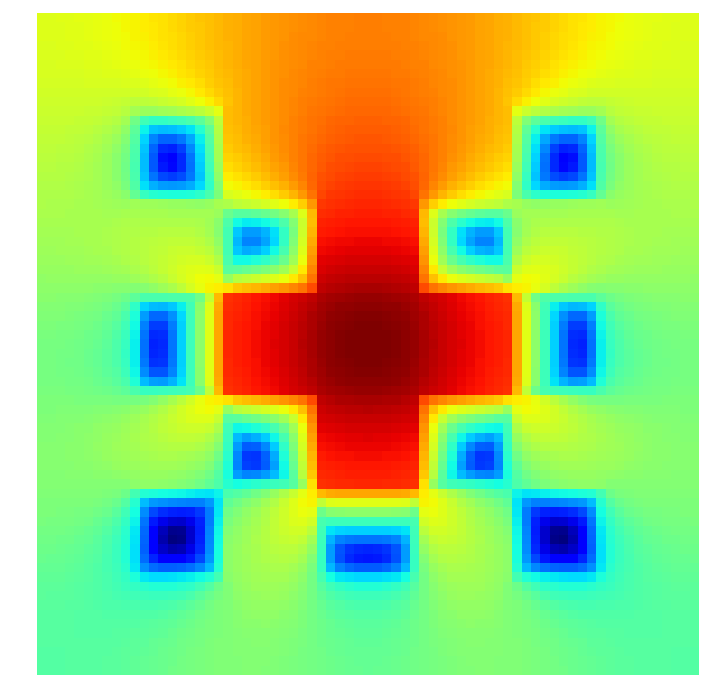
\includegraphics[width=\columnwidth]{images/checkerboard2d_p5_neumann_staggered_starmap.png}
\end{subfigure}%
\hspace{0.01\columnwidth}
\begin{subfigure}{0.49\columnwidth}
%\missingfigure{test2}
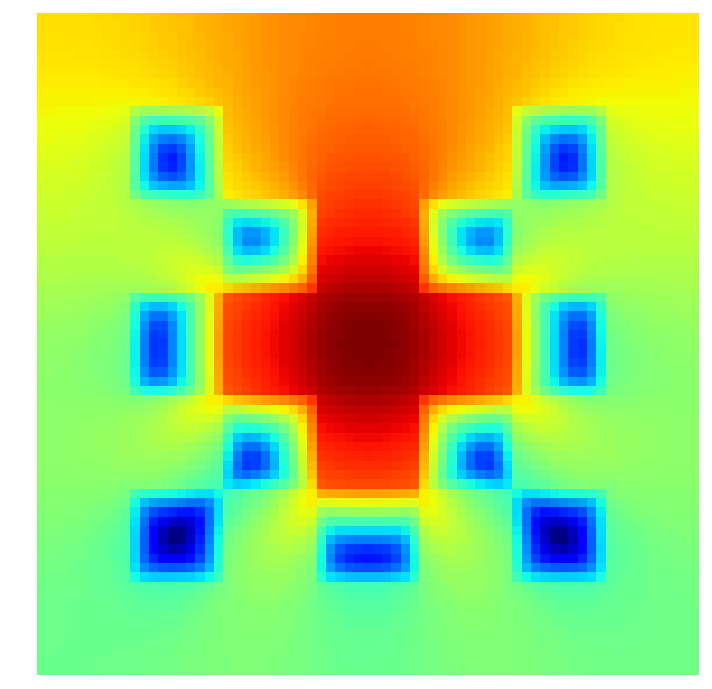
\includegraphics[width=\columnwidth]{images/checkerboard2d_p5_neumann_staggered.png}
\end{subfigure}%
\vspace{-0.1in}
\icaption{Comparison of the result for the checkerboard test using Starmap~\cite{Seibold14} (left) against ours (right). Our result is in excellent agreement with the reference. We attribute the difference at the boundary to the lack of convergence of the Starmap solve.}
\label{fig:vs_starmap}
\end{figure}

As can be seen in figure~\ref{fig:vs_starmap}, the results from our solver are in excellent agreement with the results from Seibold et al.~\cite{Seibold14} and verify the correctness of our implementation.

\subsection{Pointsource problem}

We also run our solver for the point source problem, a single point light in a homogeneous medium. This not only helps to validate our implementation for the 3D case, but also allows to get a clear assessment of the methods accuracy. We use the Grosjean approximation, which was introduced by D'Eon et al.\cite{dEon11}, as a very accurate approximation to the ground truth solution.

\begin{figure}[h]
\centering
\begin{subfigure}{0.45\columnwidth}
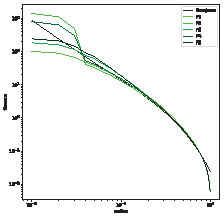
\includegraphics[width=\columnwidth]{figures/pointsource_pn.pdf}
%\missingfigure{test}
\caption{$P_N$ vs. ground truth}
\label{fig:pointsource_pn}
\end{subfigure}%
\hspace{0.05\columnwidth}
\begin{subfigure}{0.45\columnwidth}
%\missingfigure{test2}
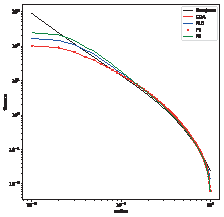
\includegraphics[width=\columnwidth]{figures/pointsource_p5.pdf}
\caption{$P_5$ vs. CDA and FLD}
\label{fig:pointsource_p5}
\end{subfigure}%
\vspace{-0.1in}
\icaption{Lineplot through the 3D solution of our solver for the point source problem for various order $N$ (left). Solution for $P_5$ compared against classical diffusion, flux-limited diffusion and analytical solution (right).}
\label{fig:pointsource}
\end{figure}

For our test case, we choose a FD resolution of $80\times80\times80$, an extinction coefficient $\sigma_t=8.0$ and albedo $\alpha=0.9$. We run the solver for different truncation values $N$. In figure~\ref{fig:pointsource}~\subref{fig:pointsource_pn}, we see that the solution becomes increasingly accurate for higher truncation order. The ground truth is underestimated when $N$ is odd, and overestimated when $N$ is even. We further see, that the $P_1$ solution exactly matches the results from CDA, which confirmes, that the latter is only a collapsed version of the former.

\subsection{Procedural Clouds}

Finally, we run our solver on different procedural cloud datasets to get an idea of its performance in more practical applications.

Figure~\ref{fig:teaser}~\subref{fig:nebulae_ours} shows the result of $P_5$ for a procedurally generated heterogeneous cloud with an isotropic phase function. We see that at order $N=5$, our method can capture indirect illumination similarily well as FLD and is significantly better than CDA as expected.

\begin{itemize}
	\item mention performance.
	\item run for various values of $N$
	\item convergence behaviour in vacuum. Clearify
	\item run for anisotropic problem
\end{itemize}


